%%%%%%%%%%%%%%%%%%%%%%%%%%%%%%%%%%%%%%%%%
% Thin Sectioned Essay
% LaTeX Template
% Version 1.0 (3/8/13)
%
% This template is based on a downloaded from:
% http://www.LaTeXTemplates.com
%
% Original Author:
% Nicolas Diaz (nsdiaz@uc.cl) with extensive modifications by:
% Vel (vel@latextemplates.com)
% and adjustments by 
% Thuy Tran 
%
% License:
% CC BY-NC-SA 3.0 (http://creativecommons.org/licenses/by-nc-sa/3.0/)
%
%%%%%%%%%%%%%%%%%%%%%%%%%%%%%%%%%%%%%%%%%

%----------------------------------------------------------------------------------------
%	PACKAGES AND OTHER DOCUMENT CONFIGURATIONS
%----------------------------------------------------------------------------------------

\documentclass[a4paper, 12pt]{report} % Font size (can be 10pt, 11pt or 12pt) and paper size (remove a4paper for US letter paper)

\usepackage[protrusion=true,expansion=true]{microtype} % Better typography
\usepackage{graphicx} % Required for including pictures
\usepackage{wrapfig} % Allows in-line images

\usepackage{mathpazo} % Use the Palatino font
\usepackage[T1]{fontenc} % Required for accented characters
\usepackage[utf8]{inputenc} 
\usepackage[ngerman]{babel}
\linespread{1.05} % Change line spacing here, Palatino benefits from a slight increase by default

\makeatletter
\renewcommand\@biblabel[1]{\textbf{#1.}} % Change the square brackets for each bibliography item from '[1]' to '1.'
\renewcommand{\@listI}{\itemsep=0pt} % Reduce the space between items in the itemize and enumerate environments and the bibliography

\renewcommand{\maketitle}{ % Customize the title - do not edit title and author name here, see the TITLE block below
\begin{flushright} % Right align
{\LARGE\@title} % Increase the font size of the title

\vspace{50pt} % Some vertical space between the title and author name

{\large\@author} % Author name
\\\@date % Date

\vspace{40pt} % Some vertical space between the author block and abstract
\end{flushright}
}

%----------------------------------------------------------------------------------------
%	TITLE
%----------------------------------------------------------------------------------------

\title{\textbf{}\\ % Title
Focused and Deliciously Witty Subtitle} % Subtitle

\author{\textsc{Alexander Beischl und Thuy Tran} % Author
\\{\textit{Technische Universität München}}} % Institution

\date{\today} % Date

%----------------------------------------------------------------------------------------

\begin{document}

\maketitle % Print the title section

%----------------------------------------------------------------------------------------
%	ABSTRACT AND KEYWORDS
%----------------------------------------------------------------------------------------

\renewcommand{\abstractname}{Zusammenfassung} % Uncomment to change the name of the abstract to something else

\begin{abstract}
Morbi tempor congue porta. Proin semper, leo vitae faucibus dictum, metus mauris lacinia lorem, ac congue leo felis eu turpis. Sed nec nunc pellentesque, gravida eros at, porttitor ipsum. Praesent consequat urna a lacus lobortis ultrices eget ac metus. In tempus hendrerit rhoncus. Mauris dignissim turpis id sollicitudin lacinia. Praesent libero tellus, fringilla nec ullamcorper at, ultrices id nulla. Phasellus placerat a tellus a malesuada.
\end{abstract}


\vspace{30pt} % Some vertical space between the abstract and first section

%----------------------------------------------------------------------------------------
%	ESSAY BODY
%----------------------------------------------------------------------------------------

\chapter{Einführung}\label{einführung}

This statement requires citation \cite{latexcompanion}; this one does too \cite{einstein}. Lorem ipsum dolor sit amet, consectetur adipiscing elit. Aenean dictum lacus sem, ut varius ante dignissim ac. Sed a mi quis lectus feugiat aliquam. Nunc sed vulputate velit. Sed commodo metus vel felis semper, quis rutrum odio vulputate. Donec a elit porttitor, facilisis nisl sit amet, dignissim arcu. Vivamus accumsan pellentesque nulla at euismod. Duis porta rutrum sem, eu facilisis mi varius sed. Suspendisse potenti. Mauris rhoncus neque nisi, ut laoreet augue pretium luctus. Vestibulum sit amet luctus sem, luctus ultrices leo. Aenean vitae sem leo.

Nullam semper quam at ante convallis posuere. Ut faucibus tellus ac massa luctus consectetur. Nulla pellentesque tortor et aliquam vehicula. Maecenas imperdiet euismod enim ut pharetra. Suspendisse pulvinar sapien vitae placerat pellentesque. Nulla facilisi. Aenean vitae nunc venenatis, vehicula neque in, congue ligula.

%------------------------------------------------

\section*{R}\label{r}
R ist eine Programmiersprache und eine Entwicklungsumgebung, die für statistische Berechnungen und Graphen unter John Chambers von Bell Laboratories entwickelt wurde. Sie ist ein GNU-Projekt, bei dem die Entwicklung von freier Software im Mittelpunkt steht. R weist große Ähnlichkeiten zu der Programmiersprache S auf, ein weiteres GNU-Projekt, welches weitgehend auch unter R läuft. \cite{rproject}

R bietet standardmäßig alle Hauptfunktionen an für die statistische Analyse von Datensätzen an und ist einfach zu erweitern, weswegen es vor allem für wissenschaftliche Arbeiten verwendet wird. Es ist mit R einfach, statistische Funktionen auf große Datenmengen anzuwenden.  


%------------------------------------------------

\section*{ARX}
ARX ist eine freie Software zur Anonymisierung von medizinischen Datensätzen, die von Fabian Prasser vom Institut für medizinische Statistik und Epidemiologie an der Technischen Universität München entwickelt wurde. 


\chapter{Anwenderdokumentation}
\section{Übersicht}
Das R-Terminal dient dazu, über eine externe Schnittstelle R aufzurufen und zu bedienen. Dies soll vor allem dazu genutzt werden, um Tabellen aus ARX einzuladen und Skripte auszuführen, und gleichzeitig die im Kapitel \ref{einführung} beschriebenen Probleme zu umgehen. Das R-Terminal ist kompatibel mit Windows, der Linux Distribution Ubuntu und OS X, von denen jeweils die folgenden Versionen im Rahmen der Entwicklung getestet wurden: 

\begin{itemize}
\item Windows 10 Education (Version 1511)
\item OS X El Capitan (Version 10.11.1)
\item Ubuntu
\end{itemize}

%insert screenshot for linux and the correct ubuntu/opensuse version

In den folgenden Abschnitten werden die Grundfunktionen und zusätzliche Features des R-Terminals beschrieben. 
\section{}

\begin{figure}[htpb]
\centering
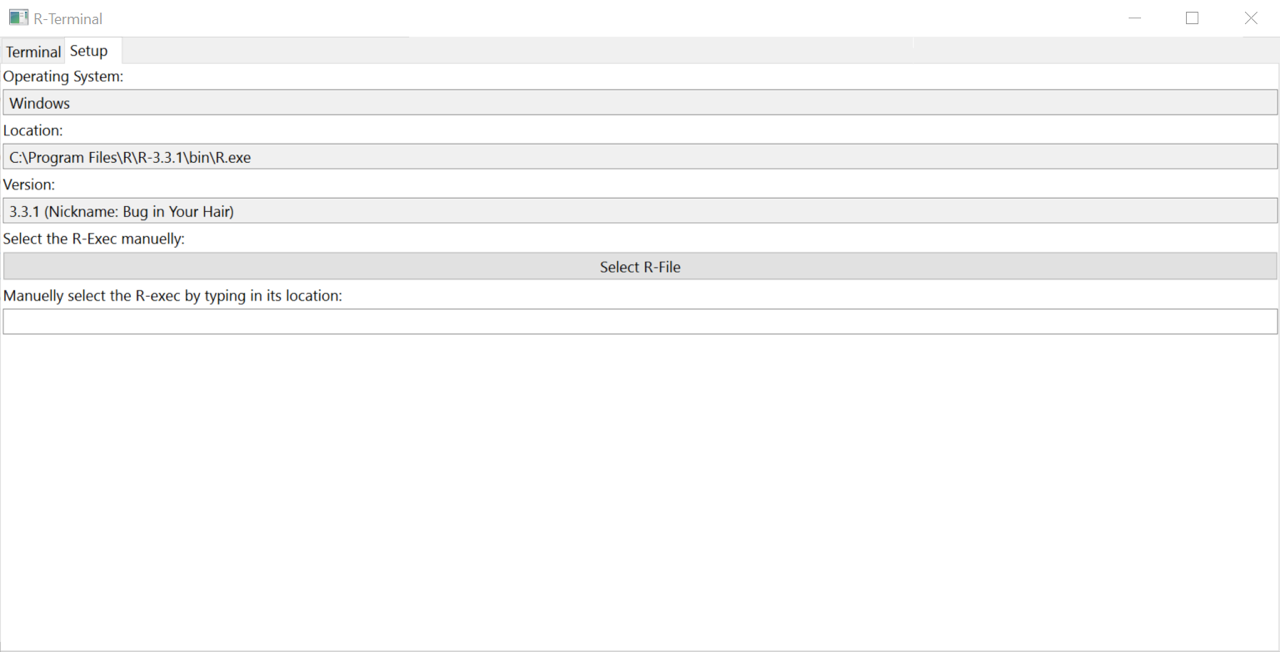
\includegraphics[width=0.8\textwidth]{R-TerminalWindows}
\caption{R-Terminal: \textit{Terminal} unter Windows 10 Education (Version 1511)}
\label{rterminalwindows}
\end{figure}

\begin{figure}[htpb]
\centering
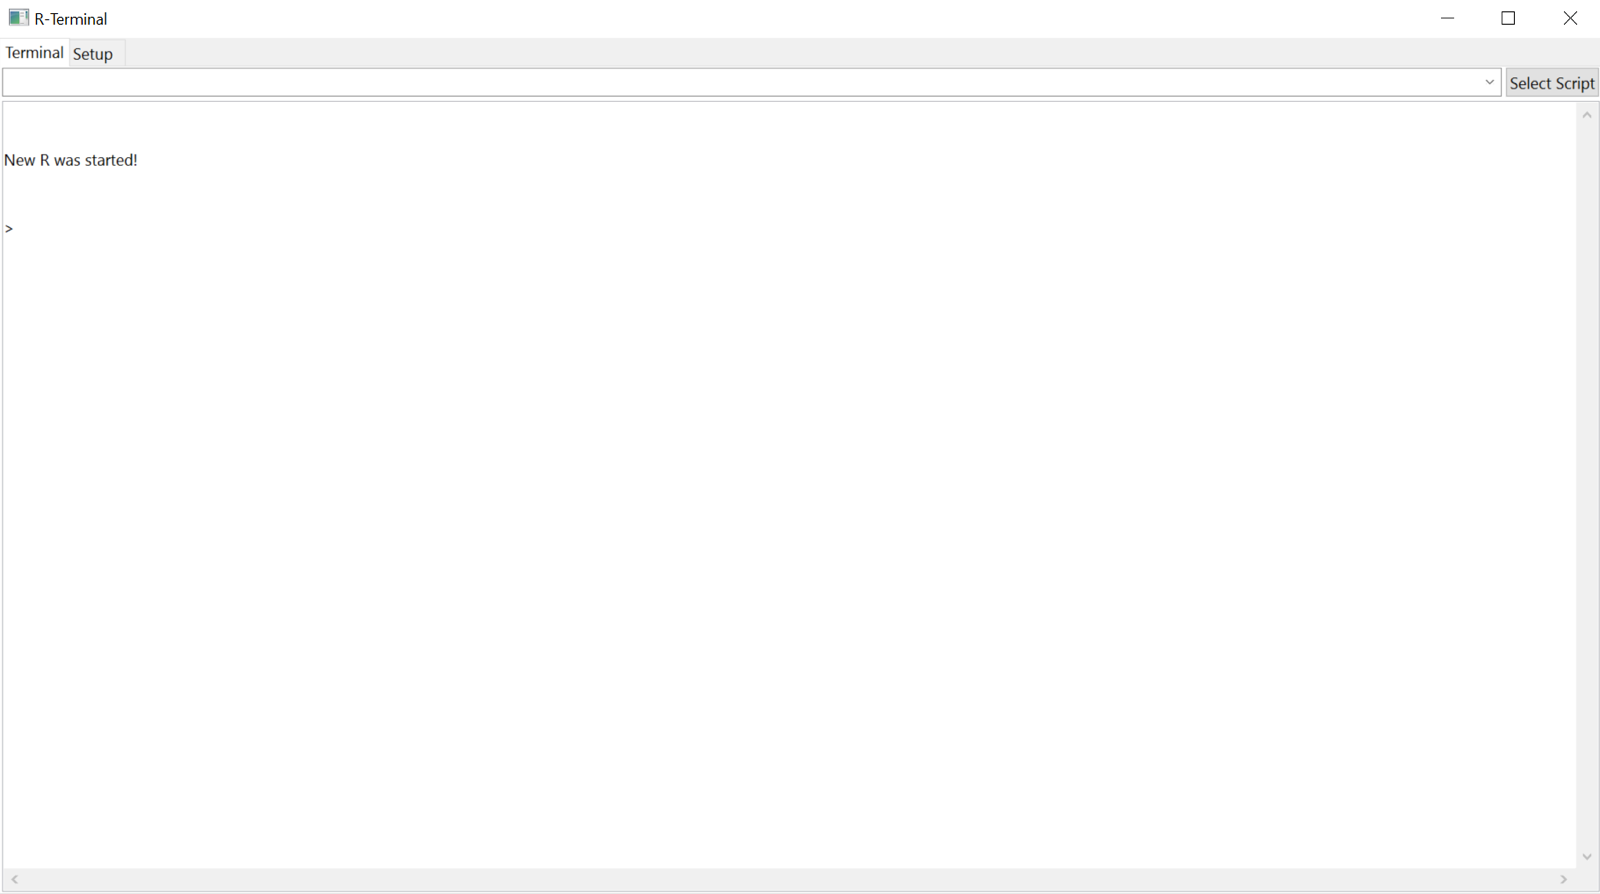
\includegraphics[width=0.8\textwidth]{rterminalwindows}
\caption{R-Terminal: \textit{Setup} unter Windows 10 Education (Version 1511)}
\label{rterminalwindows}
\end{figure}

\begin{figure}[htpb]
\centering
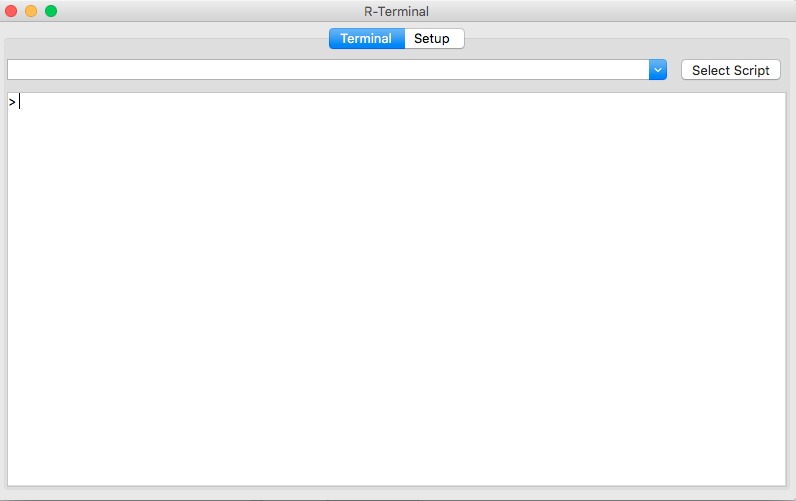
\includegraphics[width=0.8\textwidth]{R-Terminal}
\caption{R-Terminal: \textit{Terminal} unter OS X (Version 10.11.1)}
\label{rterminalmac}
\end{figure}

\begin{figure}[htpb]
\centering
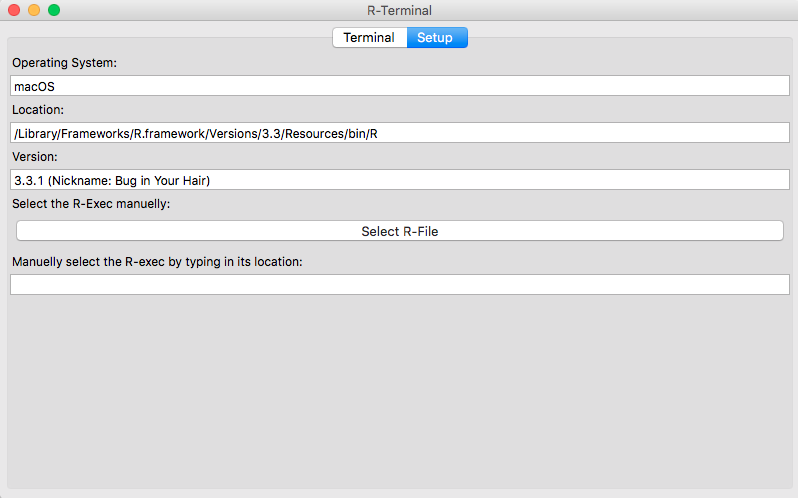
\includegraphics[width=0.8\textwidth]{rterminalsetup}
\caption{R-Terminal: \textit{Setup} unter OS X (Version 10.11.1)}
\label{macsetup}
\end{figure}

In Abbildung \ref{rterminalmac} ist das R-Terminal unter OS X (hier Version 10.11.1) zu sehen. Das Terminal verfügt über die beiden Tabs \textit{Terminal} und \textit{Setup} (s. \ref{macsetup)}. Unter \textit{Setup} wird entweder eine R-Version auf dem Rechner gesucht und automatisch ausgeführt oder es wird vom Benutzer selber der Pfad zu der gewünschten R-Version angegeben. 
\chapter{Entwicklerdokumentation}
\section{SWT}


%----------------------------------------------------------------------------------------
%	BIBLIOGRAPHY
%----------------------------------------------------------------------------------------

%\bibliographystyle{unsrt}

%\bibliography{sample}
\begin{thebibliography}{9} %Das ist nur ein Beispiel, 1 und 2 sind im dummy text oben eingebunden 
\bibitem{latexcompanion} 
Michel Goossens, Frank Mittelbach, and Alexander Samarin. 
\textit{The \LaTeX\ Companion}. 
Addison-Wesley, Reading, Massachusetts, 1993.
 
\bibitem{einstein} 
Albert Einstein. 
\textit{Zur Elektrodynamik bewegter K{\"o}rper}. (German) 
[\textit{On the electrodynamics of moving bodies}]. 
Annalen der Physik, 322(10):891–921, 1905.

 
\bibitem{rproject}
\texttt{https://www.r-project.org/about.html}
\end{thebibliography}
%----------------------------------------------------------------------------------------

\end{document}